\documentclass[letterpaper,10pt]{article}
\usepackage[margin=0.75in]{geometry}
\usepackage{graphicx}

\title{Not Exactly the Internet of Things for Outdoor Lighting:\\Progress Report}
\author{Oregon State University CS Senior Capstone Group 22\\
Malcolm Diller, Sean Rettig, Evan Steele\\
Client: Victor Hsu}
\date{\today, Fall Term}

\begin{document}

\maketitle

\section{Abstract}

Our group has made serious progress in the project to turn the Raspberry Pi and
ESP8266 Wifi module into a "Not exactly IoT" device for controlling binary
devices wirelessly. From project assignment to week five, our group produced a
proof-of-concept for the final project, and planning the final software
approach in the meantime. Despite all the writing requirements this term, we
made excellent progress.

Throughout the term, our team moved between early prototyping and detailed
documentation for the project. With regular communication through email and IRC
our group kept coordinated throughout the term, publishing progress reports to
the Sharepoint site and code samples to our Github page. We will discuss our
weekly progress and describe how the prototype and documentation unfolded over
the course of the first term of the capstone project. This should provide an
assessment on where our groups stands in preparedness to move forward with
implementation next term.

\pagebreak

\section{Weekly Breakdown}

\subsection{Weeks 0/1}

As we had not yet received our project or group assignments, we have little to
report for weeks 0 and 1.

\subsection{Week 2}

Our first week of our capstone project, ``Not exactly the Internet of Things
for Outdoor Lighting'', was relatively uneventful, as we had just received our
project and group assignments.  We met with our group promptly to create our
draft of the Problem Statement, which was largely involved expanding upon our
client's original project proposal with additional clarification, focus,
technical details, and performance metrics.

\subsection{Week 3}

During week 3, we had another group meeting to brainstorm a list of clarifying
questions to ask our client, Victor, about the project.  Having met later in
the week, we were able to get some answers:

\begin{itemize}
    \item How is the system going to be controlled by phones?  Is a dedicated
        app necessary, or can we provide a mobile-friendly website?\\ Answer: A
        mobile-friendly website is acceptable.
    \item Are we just going to be controlling lights, or are we going to expand
        to other devices if we have time (e.g. sprinkler system, music players,
        garage door openers, alarm systems)?\\
        Answer: The control of other devices is currently outside the scope of
        this project, but can be a stretch goal.
    \item Will the code for this project be open source?\\
        Answer: Yes!  The entire project is hosted on Github.com in a public
        repository.
    \item What hardware will we have access to?\\
        Answer: In addition to the hardware mentioned in the client's original
        project proposal, Victor agreed to order a 2.8" TFT Display with
        Resistive Touchscreen <http://www.adafruit.com/products/1774> for use
        with the Raspberry Pi in the control unit.
\end{itemize}

With the clarifications and direction provided by our client, we were able to finish our Problem Statement document.

\subsection{Week 4}
 
Having not received the hardware from our client yet, there was not much we
could do on the physical side.  We did, however, begin work on our Requirements
Document, listing out several core requirements, as well as some stretch goals.
Much of this work was simply listing out each individual piece of the system,
all the while filling in assumptions with explicit requirements and providing
examples to ensure the requirements cannot be misconstrued.  For some of the
aspects that we not yet sure of, we injected a little of our own vision,
knowing that our client would be able to make the final decisions on details
later.  For organizational purposes, we decided to break up the requirements
into three categories:

\begin{enumerate}
    \item Device control
    \item User interface
    \item Rules
\end{enumerate}

The ``device control'' section includes the bare essentials for booting each
device, running the control programs, and ensuring that the devices are able to
communicate with each other wirelessly.

The ``user interface'' section includes requirements regarding the user's
experience and access through the touchscreen and web site interfaces,
including how they can view, name, group, toggle, and apply rules to lights.

The ``rules'' section, then, describes the rules that will be available for
users to control their lights with.  These include time-based rules (e.g.
turning on at 8pm and off at 6am every weekday) and of course, the crowning
feature, rules for toggling based on the sunset and sunrise, obviating the need
to manually adjust the system when the sunset and sunrise times change with the
seasons.

We also included a ``stretch goals'' category following the same 3-section
layout as described above, where we filled in interesting ideas that we and our
client had, but were not absolutely necessary for the proper functioning of the
system and would only be implemented after the core requirements were complete,
if time allowed.

In the device control section, stretch goals included potentially expanding the
system to control devices other than lights, such as garage door openers, music
players, holiday decorations, and sprinklers.

In the user interface section, we considered additional usability features,
such as allowing the web interface to be accessible over the Internet (for
remote control) or even external "cloud" hosting for the web interface to
improve uptime and obviate the need for the user to port forward on their
router.

The rules section included more complex rules, such as toggling based on
weather/celestial conditions (which might require Internet access) or various
attachable sensors, such as motion sensors, light sensors, moisture sensors,
and sound sensors.  These types of rules would require significant additional
hardware, but would allow the system to, for example, turn on lights when you
pull into the driveway.  The usefulness of these rules would also greatly
increase if combined with other stretch goals, like sprinkler system control,
as the system could then be configured to stop sprinkling if the ground is
already wet (e.g. due to rain) or to pause temporarily if someone is walking
by.

\subsection{Week 5}

This week, we completed our requirements document and began researching the
hardware once we had it in our hands. We picked up the Raspberry Pi and TFTLCD
display from Victor and booted the device with the \textit{fbtft} module for
the device. This week was otherwise uneventful with everyone working on other
projects and midterms, but there was still work done with regards to group
logistics and future planning. We planned to continue our proof of concept
project next week to get the firmware and relay online.

\subsection{Week 6}
 
Most of what we did on week 6 of our project involved trying to get a
functioning proof of concept for our project, which turned out to be filled
with more problems than anticipated. We began to investigate software packages
and technologies that would help us meet the requirements outlined in our
requirements document. The main problem that we ran into this week was with the
wireless networking that we were planning on for the Pi.

We tested the devices with various wireless networking methods, including
ad-hoc and access-point mode. While testing, we discovered that the ad-hoc
system was not working as expected. This was due to the USB WiFi adapters we
were using not being compatible with an ad-hoc setup. This was especially
problematic because our main plan was to use ad-hoc for networking. After
further investigation, it became clear that we would have to reevaluate our
network implementation, as there would be no way to work around the issue and
still use ad-hoc. We are now just using the Pi as a wireless access point that
the plug nodes will connect to. This solves the problems caused by the
compatibility issues with ad-hoc.

In addition to working on the proof of concept, we also made headway on some of
the documents that we had due soon. We started an outline of our Technical
Review document, and also started revising our Requirements Document as Kevin
suggested.  We asked our TA, Xinze, to see if he had any comments on it.  His
advice was to elaborate more on the requirements we already had and make them
as specific as possible. Following his advice, we expanded on our current
requirements by adding more detail and specifying exactly what we meant, rather
than relying on assumptions.

Finally, we also wrote the first draft of our elevator pitch, a 30-second
overview of our project that we will be presenting to the rest of the class
later in the term.

\subsection{Week 7}  

After much delay, sweat, and tears, we finally had a functional proof of
concept to demo and show off. The program was quite simple, but accomplished
the bare minimum of what we would expect the program to do.  Sending a basic
TCP command to the ESP8266 module will cycle the lights through the device's
Lua firmware, and will in turn flip the relays out of the board's GPIO once we
wire it up too. The TCP commands are sent by the Raspberry Pi using a boot
script on lxTerminal, using an execution sequence that looks like this:

\begin{enumerate}
    \item Pi boots into the TFTLCD module, screen initialized
    \item Pi loads lxTerminal, runs startup script in init.d
    \item inid.d script connects to the ESP8266 module, gets an IP
    \item After the connection is made, the inid.d script starts a Python
        script
    \item The Python script cycles through TCP commands and send them to the
        device
\end{enumerate}

For our next step, we planned to make sure that the Pi could reliably perform
the discovery operation (the IP was hard-coded) and that the ESP8266 module
could run as a client in the future, connecting to the Pi to take advantage of
the Pi's DHCP server and to simplify future connections.

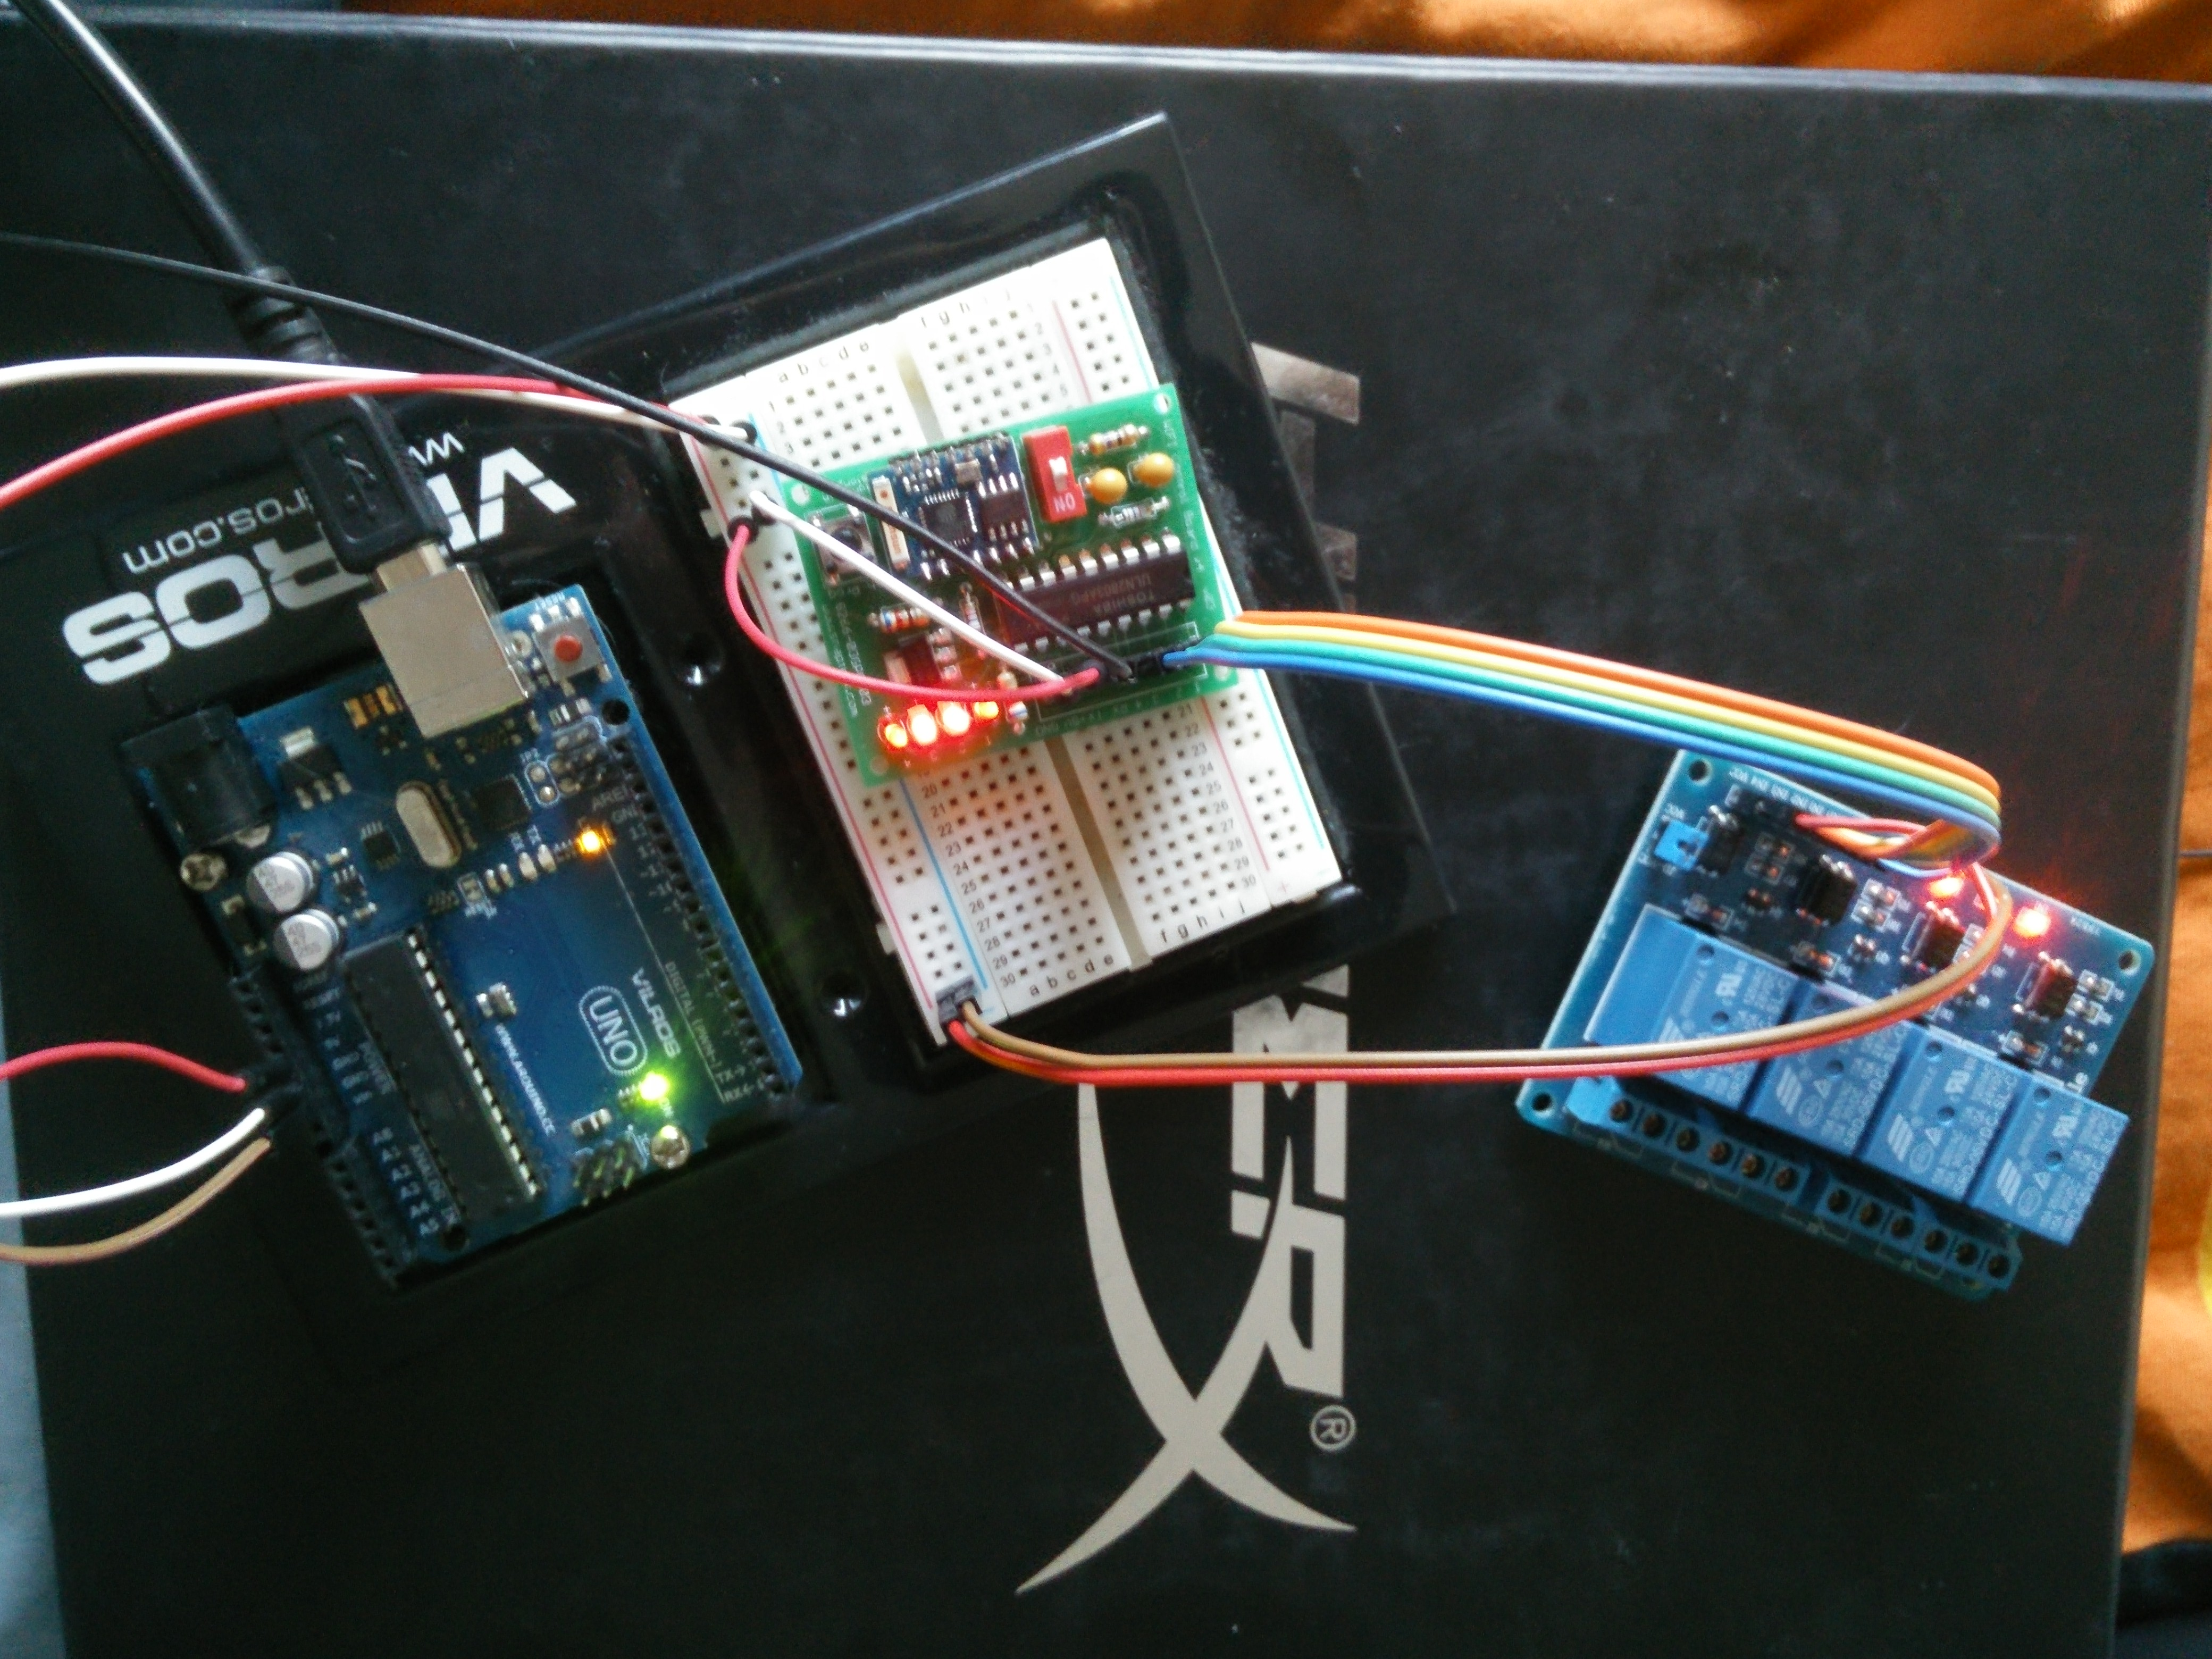
\includegraphics[scale=0.1]{circuit.jpg}

As far as documents go, we also finished revising our requirements document,
fleshed out our technology review, and started on our expo poster this week.
The expo poster largely involved filling out the provided template with the
proper information from our existing documents in a more condensed and less
technical format.

For our technology review, we chose to focus on four different main components of the system:

\begin{itemize}
    \item OS for the control unit (the Raspberry Pi)
    \item Server program implementation
    \item Web site implementation
    \item Server/client communication
\end{itemize}

For each component, we reviewed 3 potential solutions and chose what seemed to
be the best fit for the job, given our requirements for the project.

For the Pi's OS, we considered using an existing OS such as OpenWRT (designed
for networking tasks) and Raspbian (designed for ease of use on the Raspberry
Pi), but in the end, we decided to go with Yocto, as it will allow us to strip
the OS down to just what we need, making the system more optimized and
responsive.  This is particularly important given the modest processing power
of the Pi and the fact that it will be facing the user directly, making
response time all the more important.

For the server program implementation, we considered writing it in a low-level
language such as C for performance benefits.  We also considered whether to use
sysfs directly to interact with hardware devices, or whether to use the libmraa
library to abstract them and make the interaction easier.  However, in the end,
we decided to go with Python for its ease of use and higher development speed.
Since the ESP8266 can run MicroPython, using Python for the Pi as well made
sense since we only have to focus on using one language.

For the website implementation, we considered several languages and frameworks,
both for the backend and the frontend.  For the frontend, there is probably no
way to get around the standard HTML/CSS/JS stack, but for the backend, we
condidered whether to write our own site from scratch using PHP/Ruby/Python, or
whether to use a framework like Ruby on Rails for Django/Flask.  In the end, we
decided on using Flask, as it is a fairly simple yet powerful web framework
written in Python, which will allow us to use Python almost everywhere for this
project and communicate easily with the server control program.

Finally, for the server/client communication, we considered three
architectures: ad-hoc, where every device would connect to every other device;
central WAP, where the Pi would act as a central Wireless Access Point and
server, with the ESP plug units connecting to it; and CAS, where every device
connects to an external server that directs the entire system.  In the end, we
decided that the CAS system would rely too heavily on external resources and
would be too difficult to maintain, while the ad-hoc system was not possible
with the given hardware.  Thus, we decided to use the central WAP method.

\subsection{Week 8}
 
We have accomplished the task of automatic communication between the control
and plug units; booting the Pi connects it to the ESP automatically and cycles
the lights on the relay.  We also demonstrated our proof of concept to our TA,
Xinze Guan, so he could see our progress.

As far as documents go, we also finished up our expo poster and got feedback
from Kevin McGrath on our elevator pitch.  Though he said he liked it
personally, it was a bit too informal for a business presentation, so we
reworked it a bit to sound more professional.

\subsection{Week 9}
 
During week 9, we continued to work on testing out our proof of concept. We
managed to connect actual lights to our relay and verified that we can control
them by toggling them on and off. This is a good step toward getting a fully
working proof of concept working as it means we have most of the main parts
done, and mainly need to start working on the UI of the touchscreen and web
page.

We decided that we are most likely going to use Flask to implement the website.
Flask is a micro-framework for Python that is designed for developing websites.
The main reason we are planning on using it is that we are using Python for
many of the other parts of the project, and so it would be easy to integrate
this and also would make sense in terms of keeping the code consistent. To
prepare for when we are ready to start implementing that, we have begun
learning more about how Flask works, and how we might be able to use it to
create our our website.

We also presented our elevator pitch on this week, which went decently well.
There were no documents to turn in this week, and there was only class on
Tuesday, so there is not much else to report. Next week, we planned to iron out
the design document and work on the progress report. 

\subsection{Week 10}

The final week of the capstone project was largely uneventful as our group
began working on other final projects and studying for exams. However, we did
get some work in with regards to some project details and the work on the
design document.  This week, we took our document to the TA to get some
feedback regarding the design elements we focused on for the paper, and he was
pleased with the overall result after some vocabulary changes.  The hardware
project itself didn't get much direct attention this week, but we did wonder
about the usability of the final result, from a user perspective.  How easy
should the setup process be? Should the user have to worry about port
forwarding on the home network? According to Victor, our project sponsor, there
was no need to design an overly-simplified option. We will continue to
investigate more networking options over break.

\begin{itemize}
    \item Completed: Design Document\\
        The design document was reviewed by our group and a TA and turned in.
        we also had our weekly meeting with the TA at this time.  
    \item How complicated does the user setup portion of the project need to be
        and are there restrictions on what they should be able to do?\\
        Answer: As of now, having to reconnect to the device to reconfigure it
        is acceptable. Victor imagines that we won't have to connect so often
        that investing time into developing a complex networking option is not
        necessary.
    \item What will the project do over break?\\
        Answer: Evan will be taking the hardware home to use in his network
        testing bench, which is pretty much just a dozen microcomputers plugged
        into an old Cisco 2960x networking together. 
\end{itemize}

Over break, Evan will be experimenting with some networking strategies and
working with the web serve to flip the relay. Sean suggested that Flask would
provide a good framework, but as of now he's the only one with experience in
it, so Malcolm and Evan will need to study it. An ideal goal for the start of
Winter term would be having a working web interface that can flip the relay,
built with the Yocto build server. Even better if we have the interface up on
the TFTLCD screen, but we may save that until we get back together.

\end{document}
